\section{Introduction}
%Web advertising, the main source of commercial search engines'
%revenues mainly consists of textual ads which are ubiquitous short
%texts.
%\textit{Content search (or contextual advertising)} and
%\textit{sponsored search (paid search advertising)} are the mainly
%two kinds of channels for distributing such ads.
%In this paper, we only concentrate on sponsored search.
%Sponsored search is an interplay involving advertisers, search engines
%and users\cite{broder:relevancefeedback, broder:sponsoredsearch}:
%\textit{Advertisers} put bids on search phrases for their ads.
%\textit{Search engines} display ads that bid on user's
%query(\textit{exact match}) or its relevant variations(\textit{broad
%        match}) next to organic search results.
%\textit{Users} view and potentially click on ads.
%As a result, advertisers pay a certain amount of money for clicks on
%the ads that navigate users to \textit{landing pages} of their ads
%which is known as pay per click(PPC) pricing model.
%
%
%
%In this paper, we intend to maximize search engines' revenues from
%clicks.
%For simplicity, we only focus on selecting most relevant ads with respect
%to given query without consideration for ads' click prices.
%In this paper, we focus on selecting most relevant ads with respect
%to given query to maximize search engines' revenues from sponsored
%search.%using pay per click(PPC) model.
%Since each ad is characterized by one or more bid phrases that serve
%as keywords used to match user queries, these bid phrases directly
%affect how relevant the retrieved ads are with respect to user query.
%Since each ad is characterized by one or more bid phrases that serve
%as keywords used to match user queries, improving relevance between
%retrieved ads and submitted query is equivalent to bidding on most
%relevant keywords for ads and matching user query with most relevant bid phrases.
%Advertisers can choose one or more matching options for each
%keyword of their ads\cite{adword:tool}:
%\begin{itemize}
%\item \textit{Exact match} allows your ads to impress only for
%searches that use the identical phrase or close variations.
%For example, only queries ``free kids games'' and close variations
%such as ``free kid game'' can be used to match keyword ``free kids
%games''.
%Although keywords are targeted more precisely using exact match, it is
%challenging for advertisers to think up sufficient bid phrases for
%their ads.
%\item \textit{Broad match (or advanced match)} allows your ads to
%impress for searches on similar phrases and relevant variations.
%In contrast to exact match, queries ``educational games children'',
%   ``fun games kids'' and ``games'' are all allowed to match keyword
%   ``free kids games''.
%Broad match helps advertisers capture highest possible volume of ad
%traffic and meanwhile requires capability of search engines to match
%given query to many pre-defined bid phrases.
%\end{itemize}
%
%
%
%Thus, in order to improve sponsored search results and user
%experience, \textit{keyword suggestion (generation)} technology is widely
%used to help advertisers to find more appropriate
%keywords\cite{chen:concepthierarchy} and \textit{query expansion} is
%often used by search engines to include other related bid
%phrases\cite{wang:advertisementsearch}.
%To meet both advertisers' and search engines' needs, keyword research
%as well as those queries processing tasks are widely studied for
%decades.
Search advertising is a successful business
model\cite{chen:concepthierarchy} in the Internet Age.
It mainly consists of two advertising channels:
contextual advertising and sponsored
search\cite{wang:advertisementsearch,broder:relevancefeedback}.
The former selects and places ads on web pages based on keywords or
patterns extracted from page content\cite{wang:advertisementsearch}.
The latter displays ads which are selected to be relevant to search
query alongside organic search results.
It is an interplay involving search engines, advertisers and search
users\cite{broder:relevancefeedback}:
search engine hold auction to ``sell'' bid keywords to advertisers.
Advertisers bid on keywords which are representative for their
ads(e.g., Microsoft may bid on query ``cloud service for small company''
 for its ads on promoting Azure).
Search engine selects bidding ads for the query launched by users
to display. Users visit search results and interact with the
ads\cite{broder:relevancefeedback}.


To select advertisement candidates for a given query, generally speaking, 
there are two basic approaches: \textit{exact match}  and \textit{smart match}. 
The easiest
way is exact match, which directly uses the given input query to map
keywords bid by advertisers.
However, using exact match can only retrieve limited number of ads.
What's worse, it may fail sometimes, especially for tail queries.
On the other hand, smart match maps the query to a list of possible
bid keywords. It's complementary to exact match. 
%Since sponsored advertising has became the primary source of income
%for search engines\cite{thomaidou:onlineadvertising} over the past few
%years and the requirement to map the user query to more bid keywords.
%Many queries processing tasks(e.g., query suggestion, query expansion,
%        etc.) are extensively studied.
%The common objection for these queries processing tasks is to find a
%number of queries which are highly relevant to the given input
%query\cite{joshi:engineadvertising}.
%Generating a number of relevant queries for advertisers can help them
%to avoid missing popular bid keywords so that they are more likely to
%capture their potential customers\cite{chen:concepthierarchy}.
%It is also helpful to expand user's submitted query to match more ads
%because query defined by search user often results in finding limited
%appropriate ads\cite{wang:advertisementsearch}.









%In the realm of sponsored advertising, each ad is characterized by a
%list of bid phrases that serve as keywords used to match user queries.
To help advertisers find more relevant yet not so obvious keywords,
   \textit{keyword suggestion(generation)} technology is widely
   studied\cite{chen:concepthierarchy}.
On the other hand, \textit{query expansion} is often used by search
engines to match user query with more related bid phrases to recall
sufficient ads\cite{wang:advertisementsearch}.
Following properties of search phrases make \textit{keyword
    suggestion(generation)} and \textit{query expansion} extremely
    challenging.
\begin{itemize}
\item \textbf{Terms in a query are limited:} the average length of a query is between 2.4 and 2.7
words\cite{broder:webknowledge}.
\item \textbf{Queries are too various to be covered by pre-defined bid
phrases:} the vocabulary used by bid phrases is limited compared with that of user queries\cite{wang:advertisementsearch}.
\item \textbf{It's ads, but not search:} users choose terms intended to lead to optimal Web search
results rather than optimal ads\cite{broder:relevancefeedback}.
\end{itemize}
%All the efforts devoted to \textit{keyword suggestion} and
%\textit{query expansion} are indeed to address the following
%difficulties:
%\begin{itemize}
%\item \textit{Word mismatching problem} is more serious in the setting
%of sponsored advertising.
%Firstly, the average length of a search query is between 2.4 and 2.7
%words\cite{broder:webknowledge}.
%Secondly, the vocabulary used by bid phrases is limited compared with
%that of user queries\cite{wang:advertisementsearch}.
%Thirdly, in most cases, users choose terms intended to lead to optimal
%Web search results rather than optimal
%ads\cite{broder:relevancefeedback}.
%For instance, a foreign tourist may phrases his/her query as ``auto
%rental Los Angeles''.
%It is impossible to match it with keyword ``hire car LA'' by simply
%computing their similarity at term level.
%\item \textit{Long tail problem} bring in economic losses for both
%advertisers and search engines.
%Those tail queries although individually rare, make up a significant
%portion of the query volume.
%However, only 30\%-40\% of query volume is covered by ads because of
%the difficulty to interpret tail ones\cite{broder:sponsoredsearch}.
%For example, tail query ``patio furniture'' recalls less search
%results than popular one ``outdoor furniture'' as Fig
%\ref{fig:tailqueryexample} illustrated.
%In fact, ``patio furniture'' is a good choice for advertisers because
%it is not only relevant but also economical.
%\end{itemize}
%Because of these challenging problem, syntactic approaches suffer
%from low recall and it is difficult for latent semantic analysis(LSA)
%    approaches\cite{blei:dirichletallocation,deerwester:semanticanalysis,hofmann:semanticindexing}
%    to draw statistical conclusion.
%\textit{User behavior data} captures semantic relevance between
%search phrases.
%However, there is no sufficient such resouces for phrases that are
%seldom accessed.
%\begin{figure}
%\centering
%\label{fig:tailqueryexample}
%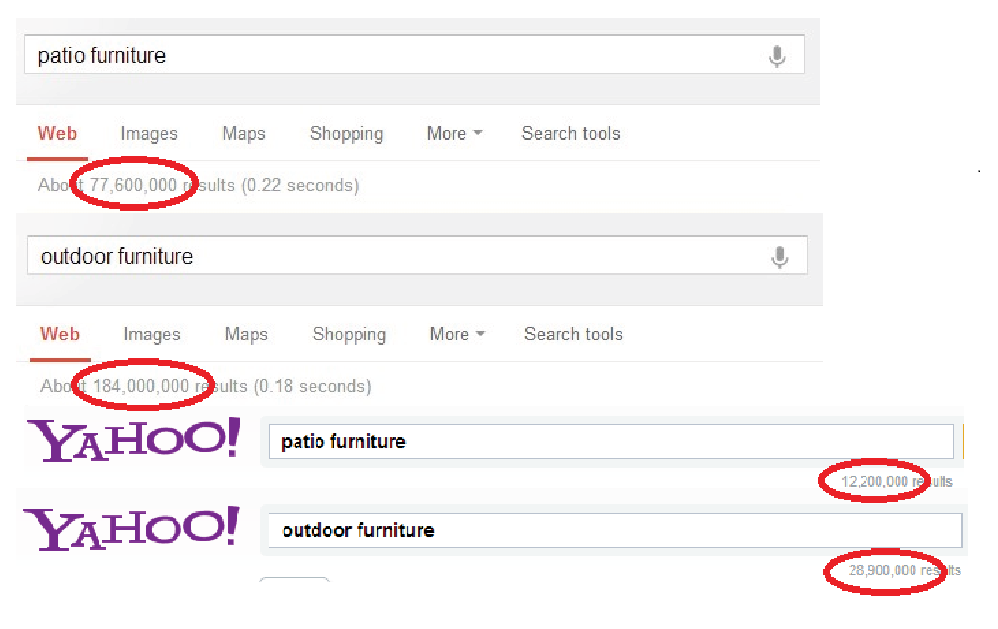
\epsfig{file=figures/example.eps,width=3.1in,height=1.9in}
%\caption{rare query and popular query}
%\end{figure}
Thus, syntactic approaches often suffer from low
recall\cite{wang:advertisementsearch}.
For instance, a tourist may phrases his/her query as ``auto rental Los
Angeles''.
It is difficult to directly match the query to keyword ``hire car LA''
through term level features.
Topic
models\cite{blei:dirichletallocation,deerwester:semanticanalysis} are
able to address such word mismatching problem well for corpus of
normal documents.
However, it is difficult for them to draw reliable statistical
conclusion from search phrases.



As Broder et al\cite{broder:webknowledge} claimed, augmenting queries
with additional external knowledge can go a long way.
%The state-of-the-art approaches can be classified according to what
%kind of external knowledges they exploit:
%\begin{itemize}
%\item \textit{Organic search results} are in most cases of high
%quality even the query is extrememly short.
%Broder et al\cite{broder:relevancefeedback} propose to enrich search phrases with contents of top-$K$ webpages retrieved by submitting that phrases to search engine.
%However, enriching queries with organic search
%results will bring in unnecessary latency and can't be applied real-time.
%\item \textit{User behavior data} captures semantic relevance between
%search phrases.
%However, there is no sufficient such resouces for phrases that are
%seldom accessed.
%\item \textit{Thesaurus and taxonomy} such as
%WordNet\cite{wordnet:tool}, wikipedia\cite{wiki:tool} and open
%directory project(ODP)\cite{odp:tool}, etc are widely
%leveraged for query expansion task.
%Gabrilovich et al\cite{gabrilovich:semanticanalysis} propose explicit semantic analysis(ESA)
%    that models search phrases as explicit concepts(title of articles) of wikipedia.
%The transformation from bag-of-words to bag-of-concepts in
%their approach is based on co-occurrence of terms within the content
%of original text snippets and terms within concepts' corresponding articles.
%%Chen et al\cite{chen:concepthierarchy} propose to suggest keywords
%%with concept hierarchy's help.
%Chen et al\cite{chen:concepthierarchy} emphasis that the performance
%of such kind of approaches is directly affected by the
%quality and coverage of adopted concept hierarchy as well as the
%precision of associating keywords with their relevant concepts.
%\end{itemize}
%Observing that even the query is very short, modern commercial search
%engines can retrieve decent organic search results which are highly
%relevant with respect to given query, Broder et
Broder et al\cite{broder:relevancefeedback} propose to enrich search phrases
with contents of top-$K$ retrieved webpages.
However, enriching queries with organic search results will bring in
unnecessary latency and can't be applied
real-time\cite{broder:sponsoredsearch}.
%User behavior data(e.g., click-through data, session data, etc.)
%    captures semantic relevance between search phrases.
Approaches\cite{cui:querylogs,broder:webknowledge,fuxman:keywordgeneration}
exploit user behavior data to capture semantic relevance between
search phrases which are significantly effective for popular queries.
However, \textit{it is harder for them to deal with queries that are seldom
accessed(Tail Queries).}
Besides, those tail queries although individually rare, make up a
significant portion of the query volume\cite{broder:sponsoredsearch}.



%the vocabulary used by bid keywords is limited compared with
%that of user queries, syntactic approaches suffer from low recall\cite{wang:advertisementsearch}.
%Such word mismatching problem is thought to be resolved by latent
%semantic
%analysis(LSA)\cite{blei:dirichletallocation,deerwester:semanticanalysis,hofmann:semanticindexing}
%but it is not the case when targeted documents are search
%phrases(around 2 terms\cite{baeza:searchengines}).
%Thus, the state-of-the-art approaches are largely expansion-based
%leveraging organic search
%results\cite{joshi:engineadvertising,broder:relevancefeedback}, user
%behavior data\cite{cui:querylogs,fuxman:keywordgeneration},
%         taxonomies\cite{chen:concepthierarchy} etc.\\
%also widely adopted to capture semantic relevance between queries.
%However, two related queries may trigger different URLs and the
%average number of URLs clicked is very low.
%user behavior data for tail queries because the volume distribution of
%web search queries follows the power law\cite{spink:theirqueries}.\\
Although short texts contain little information, human beings can
understand short texts well.
The reason lies in the rich knowledges maintained in our mental world.
Therefore, what we should provide for machines to understand short
texts automatically like humans is such knowledge.
%Motivated by this observation, thesaurus and taxonomy such as
%WordNet\cite{wordnet:tool}, wikipedia\cite{wiki:tool} and open
%directory project(ODP)\cite{odp:tool}, etc are widely adopted for
%queries processing tasks.
Motivated by this observation, Gabrilovich et al\cite{gabrilovich:semanticanalysis} propose explicit semantic
analysis(ESA) that models text snippet as explicit concepts(title of
        articles) of \textit{wikipedia}\cite{wiki:tool} which advances
a long step.
However, as Chen et al\cite{chen:concepthierarchy} pointed, the
performance of such kind of approaches is directly affected by the
quality and coverage of adopted concept hierarchy as well as the
precision of associating keywords with their relevant concepts.
The concept space of wikipedia is limited(about 111,654 concepts).
Besides, the transformation from bag-of-words to bag-of-concepts in
their approach is via \textit{loose isA} relationships---co-occurrence
of terms within the content of original text snippet and terms within
concepts' corresponding articles which is not reliable when the text
snippet is extremely short.
%%Chen et al\cite{chen:concepthierarchy} propose to suggest keywords
%%with concept hierarchy's help.
%Chen et al\cite{chen:concepthierarchy} emphasis that the performance
%of such kind of approaches is directly affected by the
%quality and coverage of adopted concept hierarchy as well as the
%precision of associating keywords with their relevant concepts.



With the similar intuition, we expand the sparse, noisy and ambiguous
input to a rich, explicit and accuracy representation via
\textit{strict isA} relationships provided by a probabilistic taxonomy
named Probase\cite{wu:manyconcepts}.
Then we can perform similarity calculation on that representation.
%In this paper, we propose a novel framework for \textit{keyword suggestion}
%and \textit{query expansion}.
%In contrast to expansion-based approaches mentioned above, we leverage
%a probabilistic taxonomy named \textit{Probase}\cite{wu:manyconcepts}.
Our \textit{conceptualization} algorithm associates each search
phrases with its relevant concepts by simple inferencing technique and
probabilities provided by Probase.
We also mine frequent patterns from the whole corpus and filter
inappropriate concepts assigned to short texts to avoid involvement of
additional noise.
%Leveraging  a probabilistic taxonomy and a entity co-occurrence
%network, we index corpus of bid phrases(both
%        popular and rare ones) by each one's relevant concepts instead
%of terms within its content.
%At runtime, we select the most similar bid phrases from indexed
%corpus as given query's suggestions(expansions) where similarity
%is measured at concept level rather than term level.
%The transofrmation from bag-of-words to bag-of-concepts in our
%approach is based on some simple inference techniques as well as several rules over
%our co-occurrence network.
%We don't have to wait for response of organic search and keep away
%from unreliable co-occurrence information between short texts and
%concepts( topics)' corresponding articles.
%Although our ranking function doesn't use conventional metrics of
%vector space model to measure similarity between short texts, we
%exploit locality sensitive hash(LSH) scheme for large scale similarity
%search to select candidates efficiently so that our framework
%possesses the scalability to handle real dataset.
%We describe our approach from perspective of the two main tasks of
%text modeling:
%\begin{itemize}
%\item \textit{Representation} of bid phrases and queries in our
%approach is explicit concepts provided by adopted taxonomy.
%Each short text snippet is modeled by explicit concepts provided by taxonomy such as Probase\cite{wu:manyconcepts}.
%To the best of our knowledge, the concept space of Probase is the
%largest among existing taxonomies.
%Besides, in contrast to existing explicit semantic analysis(ESA)
%    approaches\cite{chen:concepthierarchy,gabrilovich:semanticanalysis} which associate
%Firstly, we assign representative concepts to short text based on
%entities detected within its content.
%Then a large scale term co-occurrence network is used to do word sense
%disambiguation(WSD) so that we ensure that short text is enriched by
%appropriate semantic information without additional noise.
%Finally, we re-weight each short text's corresponding concepts
%according to their semantic functionality within the meaning of the
%short text.
%\item \textit{Ranking function} of our framework assigns score to
%short text by measuring their similarity in a ``hierarchical'' manner
%in contrast to conventional metrics used in vector model that
%measure similarity under the assumption that each coordinate is
%independent.
%In fact, we make our ranking function be able to recall bid
%phrases whose corresponding concepts are mainly parents or children
%of given query's corresponding concepts'.
%For example, customer has no idea about ``kindle'' may issue query
%``amazon ebook reader''.
%However, although ``kindle'' is more specific, it is still a so
%relevant keyword.
%Search users with identical information need but different
%extent of expertise may phrase their queries
%differently\cite{baeza:searchengines}.
%\end{itemize}
Note that our framework can be applied to general purpose text
modeling for corpus of short texts without any modifications.



We make the following salient contributions in this paper:
\begin{itemize}
\item We propose a novel expansion-based approach for \textit{keyword
    suggestion} and \textit{query expansion}.
Probase adopted in our approach has the largest concept space
among all those knowledgebases adopted by other ESA genre approaches.
With external knowledges provided by Probase, our approach can interpret
both popular and rare queries without waiting for algorithmic search.
\item We propose a robust \textit{conceptualization} algorithm.
Our algorithm map short texts into concept space via \textit{strict
    isA} relationships which is more feasible compared with
    \textit{loose isA} relationships when text snippet is very short.
Besides, our algorithm not only ``lifts'' words into their
hypernyms to resolve \textit{synonym} but also mines frequent patterns
to tackle \textit{polysemy}.
\item Our framework works not only for head queries, but also for tail queries. 
This is very critical for current ads system since selecting ads for tail queries is 
the major bottleneck. 
\item Our approach has the scalability to process real dataset
efficiently.
We implemented our approach and used it to expand 30 millions queries
with 702 millions bid phrases for a commercial search engine.
\end{itemize}


The external resources adopted in our approach are introduced in
Section 2.
In Section 3, we give a brief introduction to our system architecture.
We present our conceptualization algorithm in Section 4.
In Section 5, the process of selecting candidates and ranking
candidates to derive final results is described.
Experiments are discussed in Section 7.
We summarize related work in Section 8.
Finally, we conclude our paper in Section 9.
